% !TeX program = lualatex
% !TeX encoding = utf8
% !TeX spellcheck = uk_UA

\documentclass[
%border=1cm
]{ProblemBook}

\pagestyle{main}
%\usetikzlibrary{3d}


\usepackage{OpticsImages}




\begin{document}



%\input{difraction/difraction}


		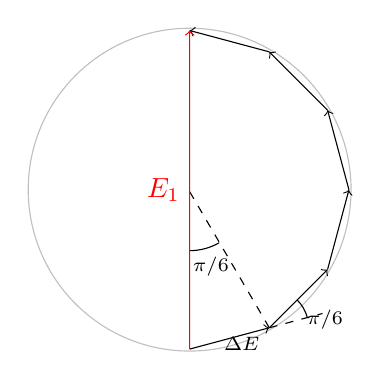
\begin{tikzpicture}
			\pgfmathsetmacro\N{6}
			\pgfmathsetmacro\m{1}
			\pgfmathsetmacro\n{\m*\N}
			\pgfmathsetmacro\E{2}
			\pgfmathsetmacro\dangle{pi*\m}
			\draw[gray!50] (0,{\E+0.025}) circle ({\E+0.05});
			\coordinate (@) at (0,0);

			\foreach[count=\j] \i in {1,...,\n}
			{

			\draw[->] (@) -- coordinate[at end] (@) ++ ({(2*\i-1)*pi/2/\N r}:{(pi*\E/\N)});

			\ifnum\j<2%
				\draw[dashed] (@) -- ++({(2*\i-1)*pi/2/\N r}:0.7);
				\draw (@) ++({(2*\i-1)*pi/2/\N r}:0.5)
				arc[start angle={(2*\i-1)*pi/2/\N r}, delta angle={2*pi/2/\N r}, radius=0.5]
				node[below right, font=\scriptsize] {$ \pi/\N $};
                \node[below left, font=\scriptsize] at (@) { $ \Delta\vect{E} $};
                \draw (0,\E) ++(0,-0.75) arc[start angle=-90, delta angle=30, radius=0.75] node[pos=0.7, font=\scriptsize, below] {$ \pi/6 $};
                \draw[dashed] (0,\E) -- (@);
			\fi
			}
			\draw[->, red] (0,0)  -- node[left] {$ \vect{E}_1 $} (@) ;
		\end{tikzpicture}


\end{document}


